Como se ha comentado anteriormente, el primer paso para monitorizar los niveles de agua tritiada es detectar los electrones que se producen en la desintegración $\beta^-$ del tritio $\eqref{desintegraciontritio}$. Para ello se utilizarán una serie de fibras centelleadoras existentes en el mercado y seleccionadas por sus características favorables para nuestro experimento~\cite{Alberto}.  Se determino que las fibras BCF-12 eran las que mejor se ajustaban a los requisitos del experimento. 

Un plástico centelleador esta formado por materiales luminiscentes cuyos átomos o moléculas que los componen presentan unos niveles energéticos similares a los de la figura \ref{Esquemafibras}:

\begin{figure}[hbtp]
\centering
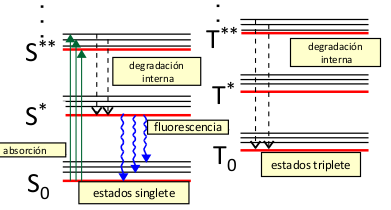
\includegraphics[scale=0.7]{EsquemaNivelesFIbras.png}
\caption{Esquema de niveles energéticos de un material centelleador~\cite{asignatura}\label{Esquemafibras}
}
\end{figure}
donde los estados $S$ representan singletes y los estados $T$ tripletes. Cuando la radiación ionizante, en nuestro caso los electrones procedentes del tritio,  atraviesan el centelleador, sus átomos y/o moléculas absorben su energía produciéndose una excitación de los mismos. 
A continuación éstos se desexcitan, en primer lugar desde niveles superiores hasta el nivel $S*$ o $T_0$ por degradación interna (en un tiempo del orden del $\pico\second$) y seguidamente del S* hasta $S_0$ (en un tiempo del orden del $\nano\second$). En esta segunda desexcitación se emiten fotones cuya longitud de onda puede ir desde el ultravioleta hasta el infrarrojo $[100-800 \nano\meter]$, dependiendo de la distancia existente entre estos niveles energéticos. La emisión de estos fotones se conoce con el nombre de  fluorescencia, y es lo que se utiliza habitualmente como señal de respuesta de un material centelleador (Fig. $\ref{Espectros}$).
Hay que tener en cuenta que las fibras centelleadoras son transparentes a los fotones que se encuentran en la longitud de onda de su emisión, ya que, de lo contrario, tendríamos una reabsorción de los fotones emitidos antes de ser detectados por el fotosensor, situación indeseada.

Los materiales centelleadoras presentan una muy buena linealidad con la energía de la radiación incidente a partir de una energía mínima, que determina la sensibilidad del material centelleador. Teniendo en cuenta que el SiPM también presenta una muy buena linealidad con la señal recibida, esperamos obtener una señal de nuestro detector que presente una buena linealidad con la energía que pretendamos medir.

Por lo general, los plásticos centelleadores producen señales bastante rápidas en comparación con otros tipos de detectores. Utilizamos fibras centelleadoras orgánicas, ya que estas son 2 o 3 órdenes de magnitud más rápidas que las inorgánicas,  en concreto, las fibras que utilizaremos presentan un tiempo de atenuación de $3.2~\nano\second$~\cite{datasheet}. Estas poseen un índice de refracción de $1.6$, parámetro fundamental a la hora de transportar eficientemente la luz.

Las fibras centelleadoras elegidas deben de producir el mayor número de fotones  posible por unidad de energía para poder tener una señal lo mayor posible. Las fibras BCF-12 son capaces de producir $8000$ fotones por $\MeV$ de la radiación incidente. Las fibras BCF-12 presentan una eficiencia de fotodetección teórica de $3.4\%$~\cite{datasheet}

Para manipular las fibras se vio necesario la utilización de guantes de látex, ya que el propio tacto  del personal encargado del tratamiento de las fibras las ensuciaban y, por extensión, la propagación de la luz se veía afectada.

Para poder cortar las fibras centelleadoras de forma ópticamente aceptable, se diseñó y construyó una guillotina adecuada en los talleres del IFIC~\cite{Alberto,anguloytiempo, dependencias, tesisfibras}, la cual se muestra en la figura~\ref{Guillotina}:

\begin{figure}[htb]
\centering
{
%\subfloat[Espectro de emisión]
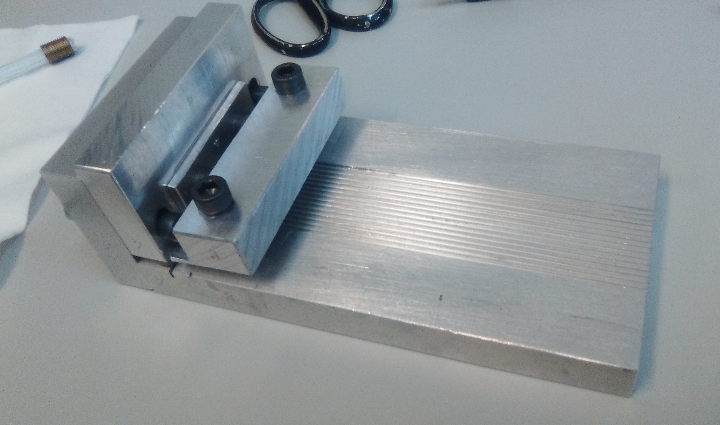
\includegraphics[scale=0.25]{Guillotina1.png} 
}
{
%\subfloat[Espectro de emisión]
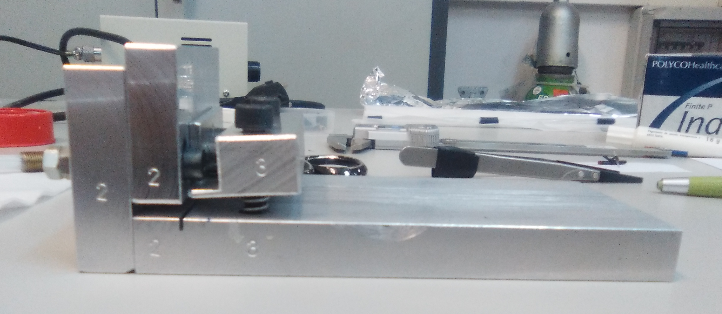
\includegraphics[scale=0.33]{Guillotina2.png} 
}
\caption{Guillotina\label{Guillotina}}
\end{figure} 

En la parte derecha se puede observar que la guillotina estaba constituida de dos piezas independientes (marcadas con los número 2 y 3), las cuales estaban suspendidas por muelles. Para sujetar y cortar cada una de las fibras, había que pulsar las piezas 3 y 2 respectivamente. 

También puede apreciarse que la guillotina dispone de 14 rieles cuadrados, los cuales servían para sujetar cada una de las fibras y, así, obtener un corte limpio y perpendicular. Aunque la guillotina tenía la posibilidad de realizar cortes simultáneos sobre varias fibras centelleadoras, siempre se realizaron cortes sobre una única fibra. De esta forma asegurábamos un mejor acabado.

Se estuvo probando con varios tipos de cuchilla (de distinto grosor y tamaño),  y se obtuvo que una cuchilla típica de afeitar era adecuada. Hay que tener en cuenta que, para un corte más efectivo, se introdujo en la disposición de la cuchilla una ligera inclinación~\cite{Alberto, anguloytiempo}. 

En la figura~\ref{Pulido} izquierda, obtenida  con ayuda de un microscopio, se puede ver  la cara de una fibra recién cortada. En ésta  figura podemos apreciar que, aunque presenta una acabado realmente bueno (sin roturas ni deformaciones), la cara de la fibra se encuentra ligeramente dañada,  lo que afecta a la propagación de la luz. La forma de subsanar este problema fue pulir cada una de las caras de las fibras. En la parte derecha de la misma figura podemos observar una foto con la misma fibra tras el proceso de pulido. Podemos comprobar que el simple hecho de pulir las caras de las fibras nos permite obtener un acabado ópticamente aceptable~\cite{Alberto, manual}.

\begin{figure}[htb]
\centering
{
%\subfloat[Espectro de emisión]
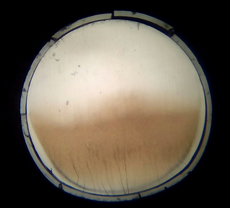
\includegraphics[scale=0.6]{SinPulir.png} 
}
{
%\subfloat[Espectro de emisión]
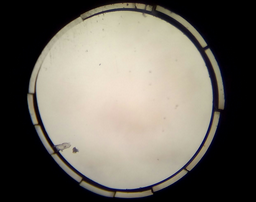
\includegraphics[scale=0.6]{Pulida.png} 
}
\caption{Cara fibras\label{Pulido}}
\end{figure} 

Hay que notar en la figura que el clad está roto. Se vio que esto era una característica inevitable del proceso de cortado. Sin embargo, pudo observarse que la ruptura únicamente se encontraba en el extremo final de la fibra, por lo que  la utilización de grasa óptica  (Saint-Gobain, BC-360) para acoplar ésta al fotosensor solucionaba el problema. 
%La grasa óptica utilizada posee un índice de refracción de 1.465, parecido al de las fibras utilizadas, 1.49.
Seguidamente, con las fibras ya cortadas, se utilizó un pegamento óptico (también de  Saint Gobain), especialmente diseñado para materiales centelleadores, para pegarlas entre ellas y obtener, de esta forma, un haz de fibras. Para que su acabado fuese suficientemente rígido se utilizó un anillo metálico en cada uno de los extremos, motrado en la figura~\ref{Arofibra}.

\begin{figure}[htb]
\centering
{
%\subfloat[Espectro de emisión]
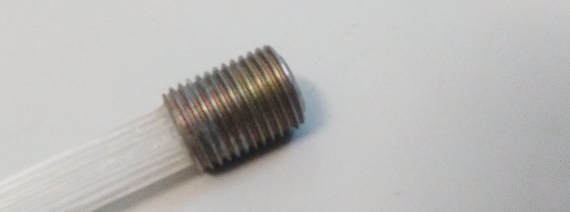
\includegraphics[scale=0.4]{arometalico.png} 
}
{
%\subfloat[Espectro de emisión]
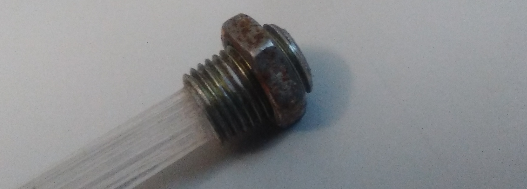
\includegraphics[scale=0.4]{arometalicoconrosca.png} 
}
\caption{Aro metálico\label{Arofibra}}
\end{figure} 

En la figura~$\ref{Arofibra}$ derecha puede apreciarse que este mismo aro disponía de una arandela la cual se utilizaba para una completa sujeción al prototipo.

Finalmente, cuando se había secado el pegamento, volvíamos a pulir cada una de las caras del haz de fibras con el objetivo de obtener una cara total plana (todas las fibras al mismo nivel) para obtener el mejor acoplamiento con el fotosensor (ya sea SiPM o PMT). En la figura~$\ref{Bunch}$ podemos observar un  haz de fibras totalmente acabado.

\begin{figure}[htb]
\centering
{
%\subfloat[Espectro de emisión]
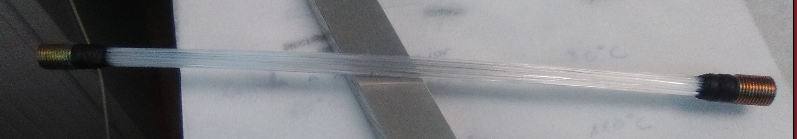
\includegraphics[scale=0.33]{bunchfibras.png} 
}
{
%\subfloat[Espectro de emisión]
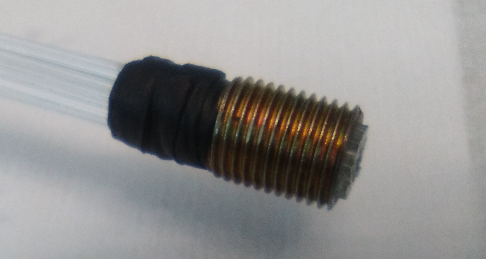
\includegraphics[scale=0.33]{bunchfibras1.png} 
}
\caption{Haz de fibras centelleadoras\label{Bunch}}
\end{figure} 

El haz  construido consiste de $35$ fibras, que es el mayor número de fibras que cabe en el interior del aro metálico y tiene una longitud de aproximadamente $25\cm$, extensión acorde con el prototipo. En la figura~\ref{Bunch} derecha podemos apreciar la cara final pulida, perfectamente plana. Hay que tener en cuenta que cualquier irregularidad inferior al milímetro en la cara final del haz es subsanada por la grasa óptica empleada para acoplar el haz de fibras al fotosensor.
